
    \begin{frame}[fragile]{Industrial Logistics}
        % \begin{center}
        % The {\bf industrial logistics}:
        % \end{center}
        \begin{columns}
            \begin{column}{.25\textwidth}
                \begin{itemize}
                \item  planning
                \item  organization
                \item  control
                \end{itemize} 
            \end{column}
            \begin{column}{.25\textwidth}
                \begin{itemize}
                    \item storage
                    \item service
                    \item costs
                \end{itemize}
            \end{column}
        \end{columns}
        \addvspace{0.6cm}
        \begin{figure}[hbt]
            \centering
            
\includegraphics[width=\textwidth]{img/ind4.png}
        \end{figure}
        {\let\thefootnote\relax\footnote{{http://www.assimpresa.org/limpresa-del-futuro-verso-industry-4-0/}}}  
    \end{frame}

    \begin{frame}[fragile]{Multi-Robot Systems for logistic applications}

        \begin{figure}[hbt]
            \centering
            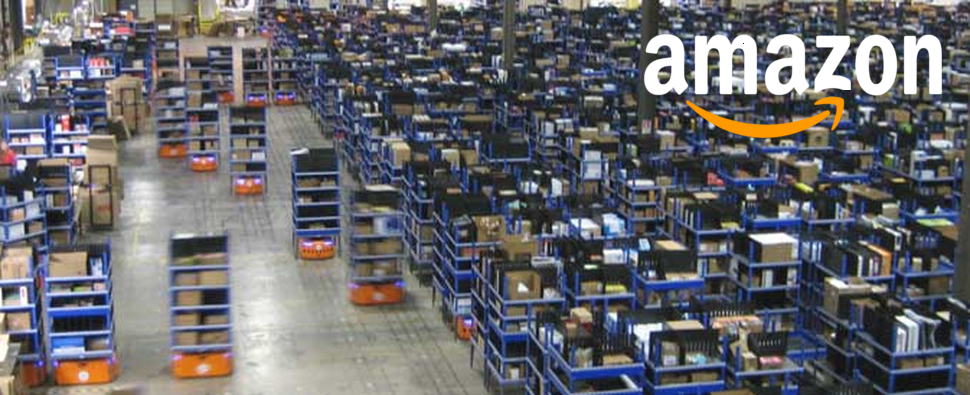
\includegraphics[width=\textwidth]{img/kiva.png}
        \end{figure}
        
        
    {\bf Kiva} warehouse-management system. 
    Focus on Multi-Robot system for robotics warehouse, allocate one task for one robot.
    {\let\thefootnote\relax\footnote{{Coordinating Hundreds of
    Cooperative, Autonomous
    Vehicles in Warehouses.}}}
    {\let\thefootnote\relax\footnote{{Lifelong Path Planning with Kinematic Constraints
    for Multi-Agent Pickup and Delivery.}}}
    \end{frame}

    \begin{frame}[fragile]{Thesis contribution}
        \begin{columns}
            \begin{column}{.7\textwidth}
            We focus on task allocation for {\bf one} robot {\bf multiple} task,            
            resolving a {\bf partition} set of task $\mathcal{T}$
            
            \begin{itemize}
                
                \item {\bf Baseline} for our experiments

                \begin{enumerate}
                    \item Single robot : Single task (SR:ST)
                \end{enumerate}

                \item Proposing two methods
                \begin{enumerate}
                    \item {\bf Set Partition Strategy} - Single robot : Multiple task (SPS1:N)
                    \item {\bf Greedy Set Partition Strategy} - Single robot : Multiple task (GSP1:N)
                \end{enumerate}
                \item {\bf real scenario}: Computer Engineering for Industry 4.0 Laboratory (ICE Lab) and  extension of  \texttt{ROS}  package
            \end{itemize}
            \end{column}
            \begin{column}{.4\textwidth}
                $+$ increasing {\bf productivity}
                
                $-$ {\bf time} and {\bf distance} travel 
            \begin{figure}
                \subfloat{
\includegraphics[scale=0.45]{img/ros}}\qquad
                \subfloat{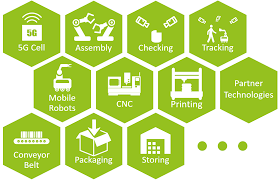
\includegraphics[scale=0.45]{img/ice}}
            \end{figure}
            \end{column}
        \end{columns}
    \end{frame}

    \begin{frame}[fragile]{ICE Laboratory}
        \begin{figure}[hbt]
            \centering
            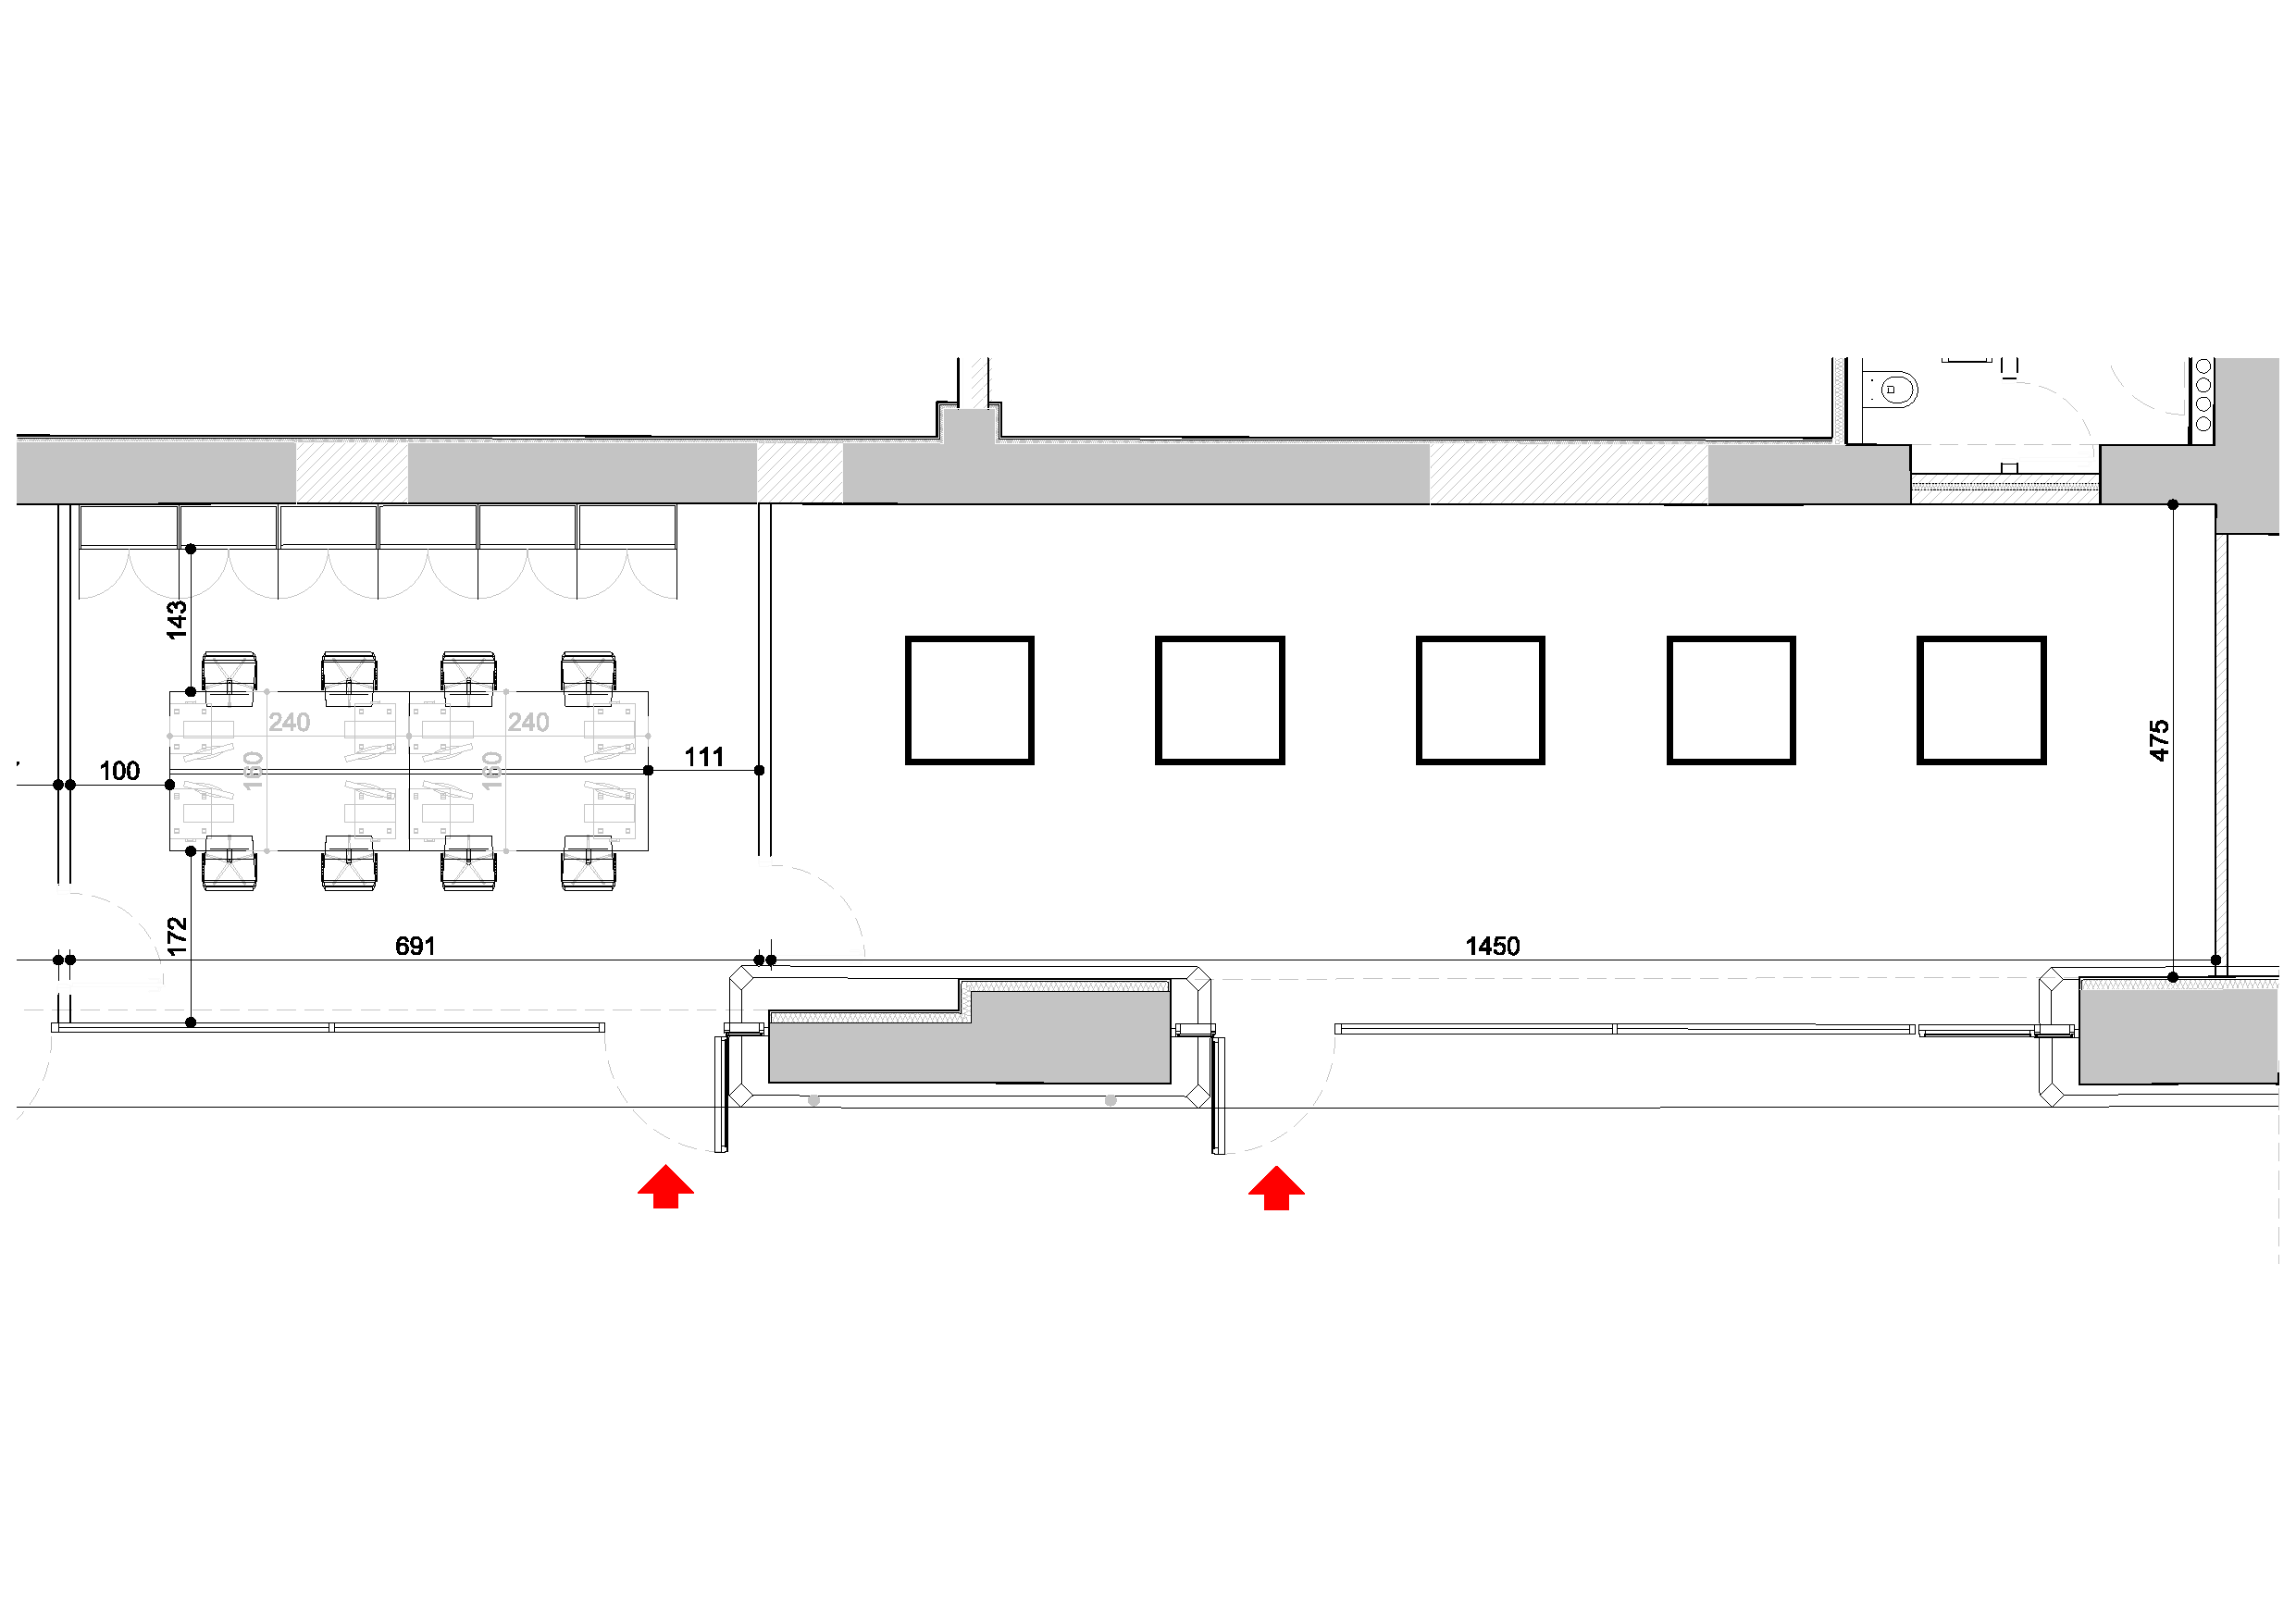
\includegraphics[width=\textwidth]{img/model1}
        \end{figure}
    \end{frame}

    \begin{frame}[fragile]{ICE Laboratory for logistic application}
        \begin{figure}[hbt]
            \centering
            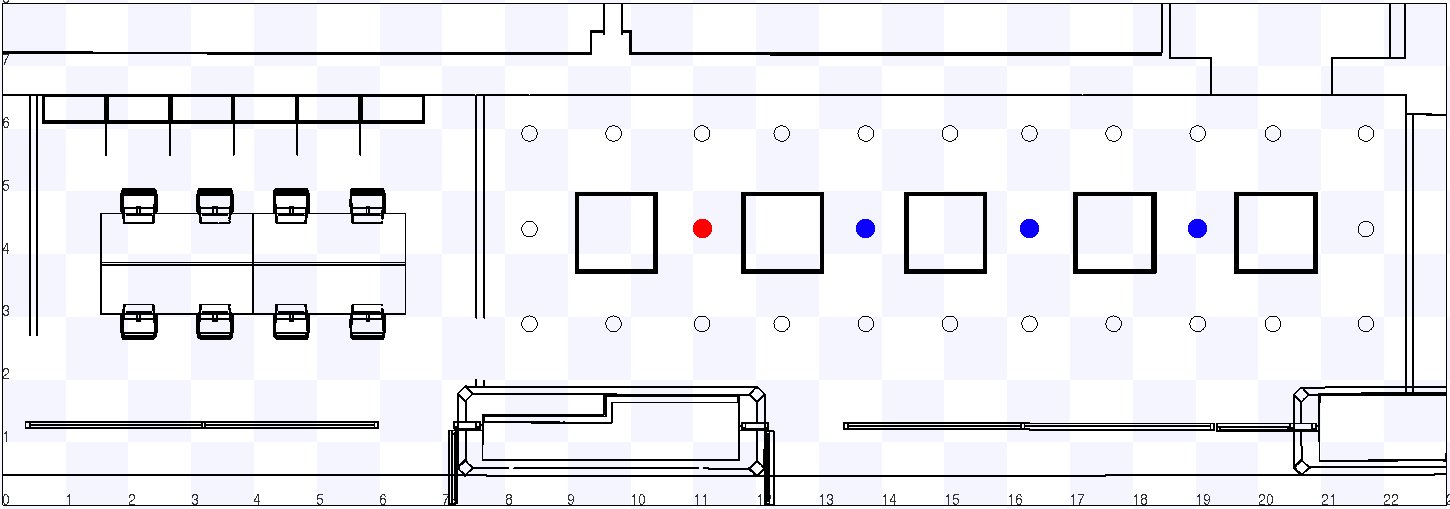
\includegraphics[width=\textwidth]{img/labgrafo}
        \end{figure}

        {\color{red}{$\bullet$}}  Loading bay
        \\
        {\color{blue}{$\bullet$}}  Unloading bays
        \\
        {\color{black}{$\circ$}}  Vertices
    \end{frame}

    \begin{frame}[fragile]{Problem formalization}
        
        Given a finite set of tasks $\mathcal{T}$, we want to compose its elements to 
        create subsets $S\subseteq\mathcal{T}$.

        \begin{figure}
            
            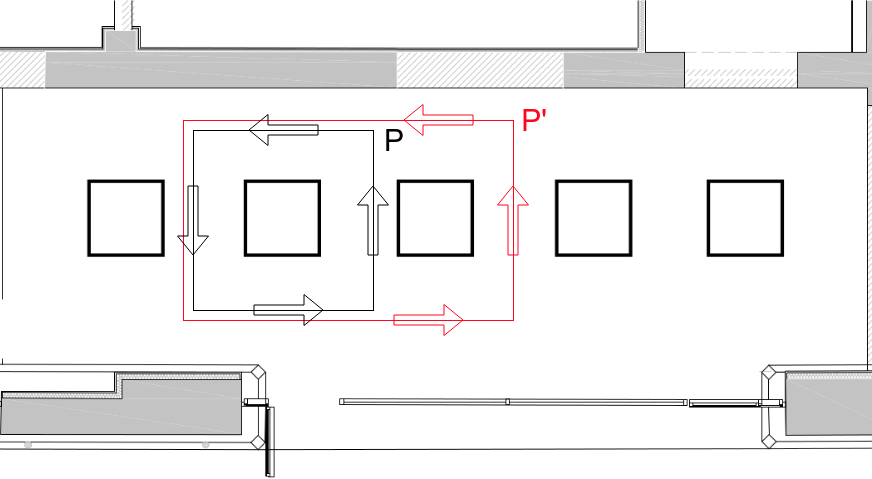
\includegraphics[scale=0.18]{img/p1p2_cut.png}
            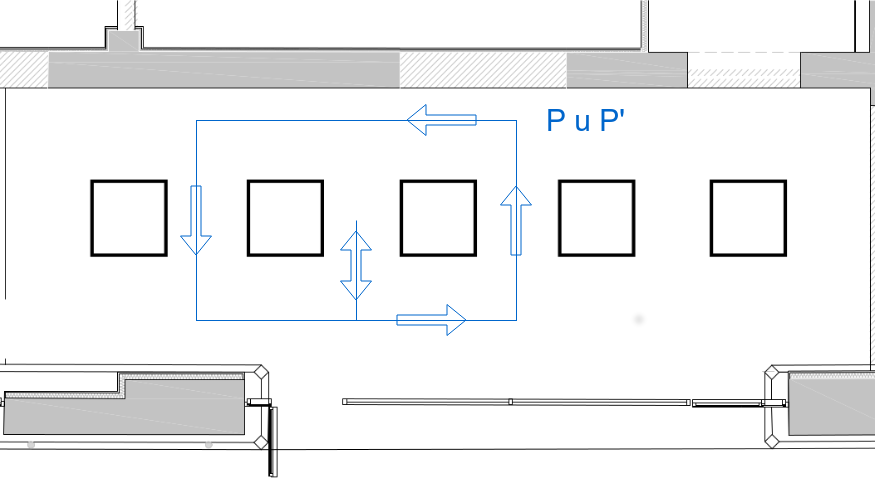
\includegraphics[scale=0.18]{img/p3_cut.png}
            
        \end{figure}
        $S = \{T_1,\cdots,T_k\}$ for each element we {\bf combine} their paths $P$ to form
        a single path $\pi = \{v_1,\cdots,v_i\}$.
    \end{frame}

    \begin{frame}[fragile]{Problem formalization 2}
       We {\bf maximize} the total demand ($d_S$).
        \[d_S =demand(T_1) + \cdots + demand(T_k)\]
        The heuristic function $v(\cdot)$ which
        can be defined for any task $T$ or subset $S$:
        \[ v(S) = \frac{f(\pi)}{d_S}\]
    \end{frame}

    \begin{frame}[fragile]{Single robot : Single task (SR:ST)}
        This method is a {\bf baseline} for our logistic scenario.

        \begin{figure}[hbt]
            \centering
            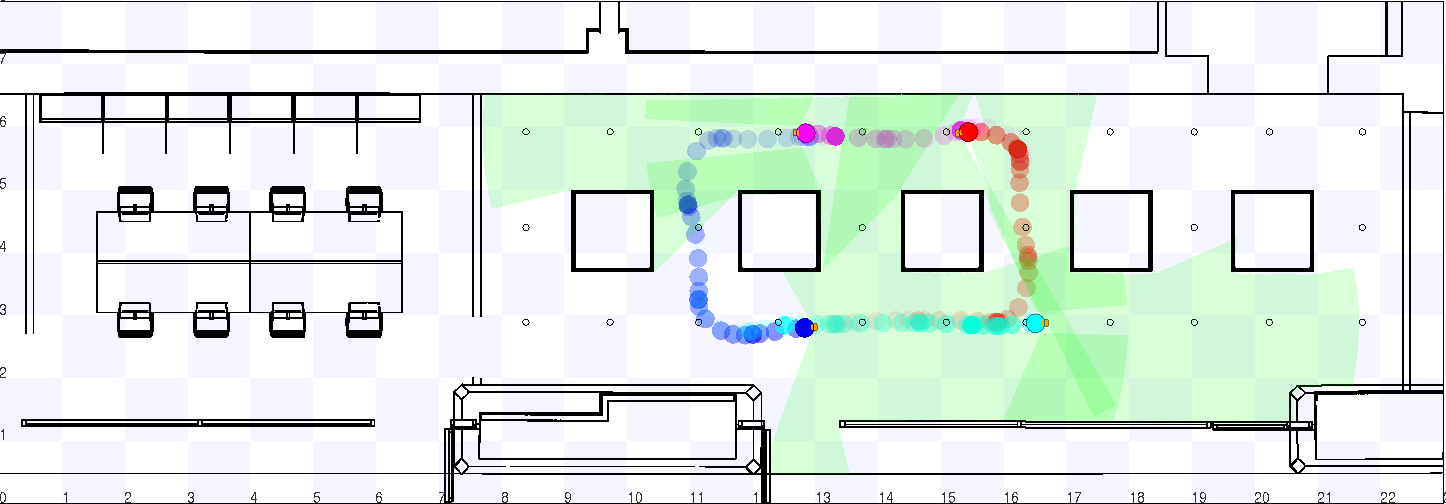
\includegraphics[width=\textwidth]{img/cycle1.png}
        \end{figure}
        The important constraint of this approach is to consider only {\bf one task} allocated for 
{\bf one robot} at time.
    \end{frame}


    \begin{frame}[fragile]{Problem formalization 3}

        For compute the {\bf best partition} the heuristic is based on the concept of {\bf loss} $L$,
        which can be defined for any pair of subset $S_i$, $S_j$ as:
        \[L(S_i,S_j) = v(\{ S_i \cup S_j\}) - v(S_i) - v(S_j)\]

        We want {\bf minimize} the cost:
        \[L(S_i,S_j) < 0 \]
    \end{frame}

    \begin{frame}[fragile]{Greedy Set Partition Strategy - Single robot : Multiple task (GSP1:N)}
        The main concept of this approach is composing tasks using Greedy {\bf Coalition Formation} strategy.
        \begin{figure}[hbt]
            \centering
            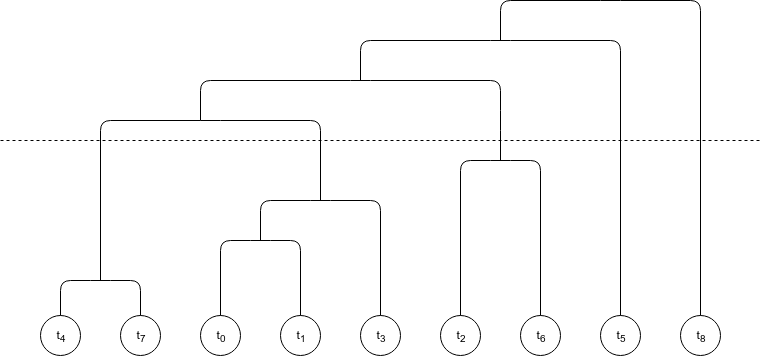
\includegraphics[width=\textwidth]{img/SP.png}
        \end{figure}
    \end{frame}


    \begin{frame}[fragile]{Set Partition Strategy - Single robot : Multiple task (SPS1:N)}
        \begin{columns}
           \begin{column}{.7\textwidth}
               \begin{center}
                   \begin{tabular}{|c|r|c|} \hline
                   \textbf{iteration} & \textbf{partition size} & \textbf{partition} \\ \hline
                   1    & 1    & \{\{a, b, c, d\}\}   \\
                   2    & 2    & \{\{a, b, c\}, \{d\}\}   \\
                   3    & 2    & \{\{a, b, d\}, \{c\}\}   \\
                   4    & 2    & \{\{a, b\}, \{c, d\}\}   \\
                   5    & 3    & \{\{a, b\}, \{c\}, \{d\}\}   \\
                   6    & 2    & \{\{a, c, d\}, \{b\}\}   \\
                   7    & 2    & \{\{a, c\}, \{b, d\}\}   \\
                   8    & 3    & \{\{a, c\}, \{b\},\{d\}\}   \\
                   9    & 2    & \{\{a, d\}, \{b, c\}\}   \\
                   10   & 2    & \{\{a\}, \{b, c, d\}\}   \\
                   11   & 3    & \{\{a\}, \{b, c\}, \{d\}\}   \\
                   12   & 3    & \{\{a, d\}, \{b\}, \{c\}\}   \\
                   13   & 3    & \{\{a\}, \{b, d\}, \{c\}\}   \\
                   14   & 3    & \{\{a\}, \{b\}, \{c, d\}\}   \\
                   15   & 4    & \{\{a\}, \{b\}, \{c\},\{d\}\}   \\ \hline       
                   \end{tabular}
                 \end{center}
           \end{column}
           \begin{column}{.4\textwidth}
            \begin{center}
           $\argmin_{P} \sum_{S \in P} v(S)$
            \end{center}
           \begin{figure}
               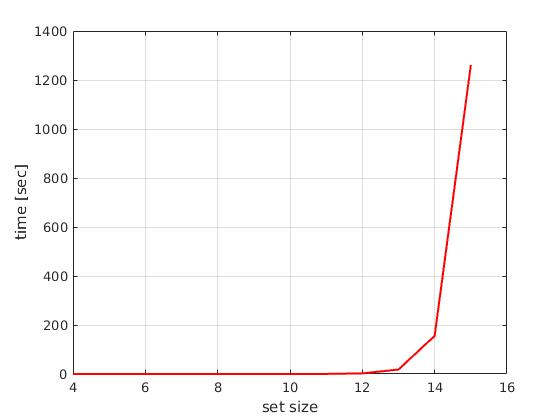
\includegraphics[width=\textwidth]{img/exp}
           \end{figure}
           \end{column}
       \end{columns}
   \end{frame}

    \begin{frame}[fragile]{Example}
        \begin{center}
        Given a set of tasks $\mathcal{T}= \{  \{T_0\}, \{T_1\}, \cdots, \{T_8\} \}$ defined like:

        ${T_i=(item, demand, unloading\_bay)}$.
        
        The agents have the {\bf same capacity} $C_{0,1,2,3} = 4$.
                    \begin{center}
                      % \centering
                      \begin{tabular}{|c|c|c|c|} \hline
                        \textbf{task} & \textbf{item} & \textbf{demand} & \textbf{unloading bay} \\ \hline
                        0    & A    & 1      & 0             \\
                        1    & B    & 2      & 1             \\
                        2    & C    & 3      & 2             \\
                        3    & A    & 1      & 0             \\
                        4    & B    & 2      & 1             \\
                        5    & C    & 3      & 2             \\
                        6    & A    & 1      & 0             \\
                        7    & B    & 2      & 1             \\
                        8    & C    & 3      & 2             \\ \hline       
                      \end{tabular} 
                    \end{center}
                    Often in the logistic environments robots are {\bf all equal}. 
                \end{center}
            
    \end{frame}

    \begin{frame}[fragile]{Example 2}
        Result SPS:
            \begin{center}
              \begin{tabular}{|c|c|c|c|} \hline
              \textbf{task} & \textbf{item} & \textbf{demand} & \textbf{unloading bay} \\ \hline
              \{4,7\}    & B    & 4     & 1             \\
              \{0,1,3\}  & \{A,B\}& 4    & \{0,1\}             \\
              \{2,6\}    & \{C,A\}    & 4  & \{0,2\}             \\
              5    & C    & 3      & 2             \\
              8    & C    & 3      & 2             \\ \hline       
              \end{tabular}
              
            \end{center}
        Result GSP:
            \begin{center}
              \begin{tabular}{|c|c|c|c|} \hline
              \textbf{task} & \textbf{item} & \textbf{demand} & \textbf{unloading bay} \\ \hline
              \{3,2\}    & \{A,C\}    & 4     & \{0,2\}             \\
              \{0,1\}    & \{A,B\}    & 3     & \{0,1\}             \\
              \{6,4\}    & \{A,B\}    & 3     & \{0,1\}             \\
              5    & C    & 3      & 2             \\
              8    & C    & 3      & 2             \\        
              7    & B    & 2      & 1             \\\hline
              \end{tabular}
              
            \end{center}
       
    \end{frame}


    \begin{frame}[fragile]{Empirical Methodology}
       
        \begin{columns}
            \begin{column}{.5\textwidth}
                Robot Operating System - \texttt{ROS}:
                \begin{itemize}
                    \item hardware abstraction 
                    \item low-level device control
                    \item message-passing
                    \item package management
                \end{itemize}
            \end{column}
            \begin{column}{.55\textwidth}
                \texttt{Stage 2D} simulator:
                \begin{itemize}
                    \item virtual world
                    \item mobile robots 
                    \item sensors, localization and actuators
                    \item realistic
                \end{itemize}
            \end{column}
        \end{columns}
        \addvspace{0.6cm}
        Probabilistic {\bf localization} technique \texttt{amcl} (Adaptive Monte Carlo Localization).
       
        {\bf Navigation} purpose we rely on \texttt{move\_base} package which create an interface with \texttt{ROS} navigation stack.
    \end{frame}

    \begin{frame}[fragile]{ROS package Logistic\_sim}
        \begin{figure}[hbt]
            \centering
            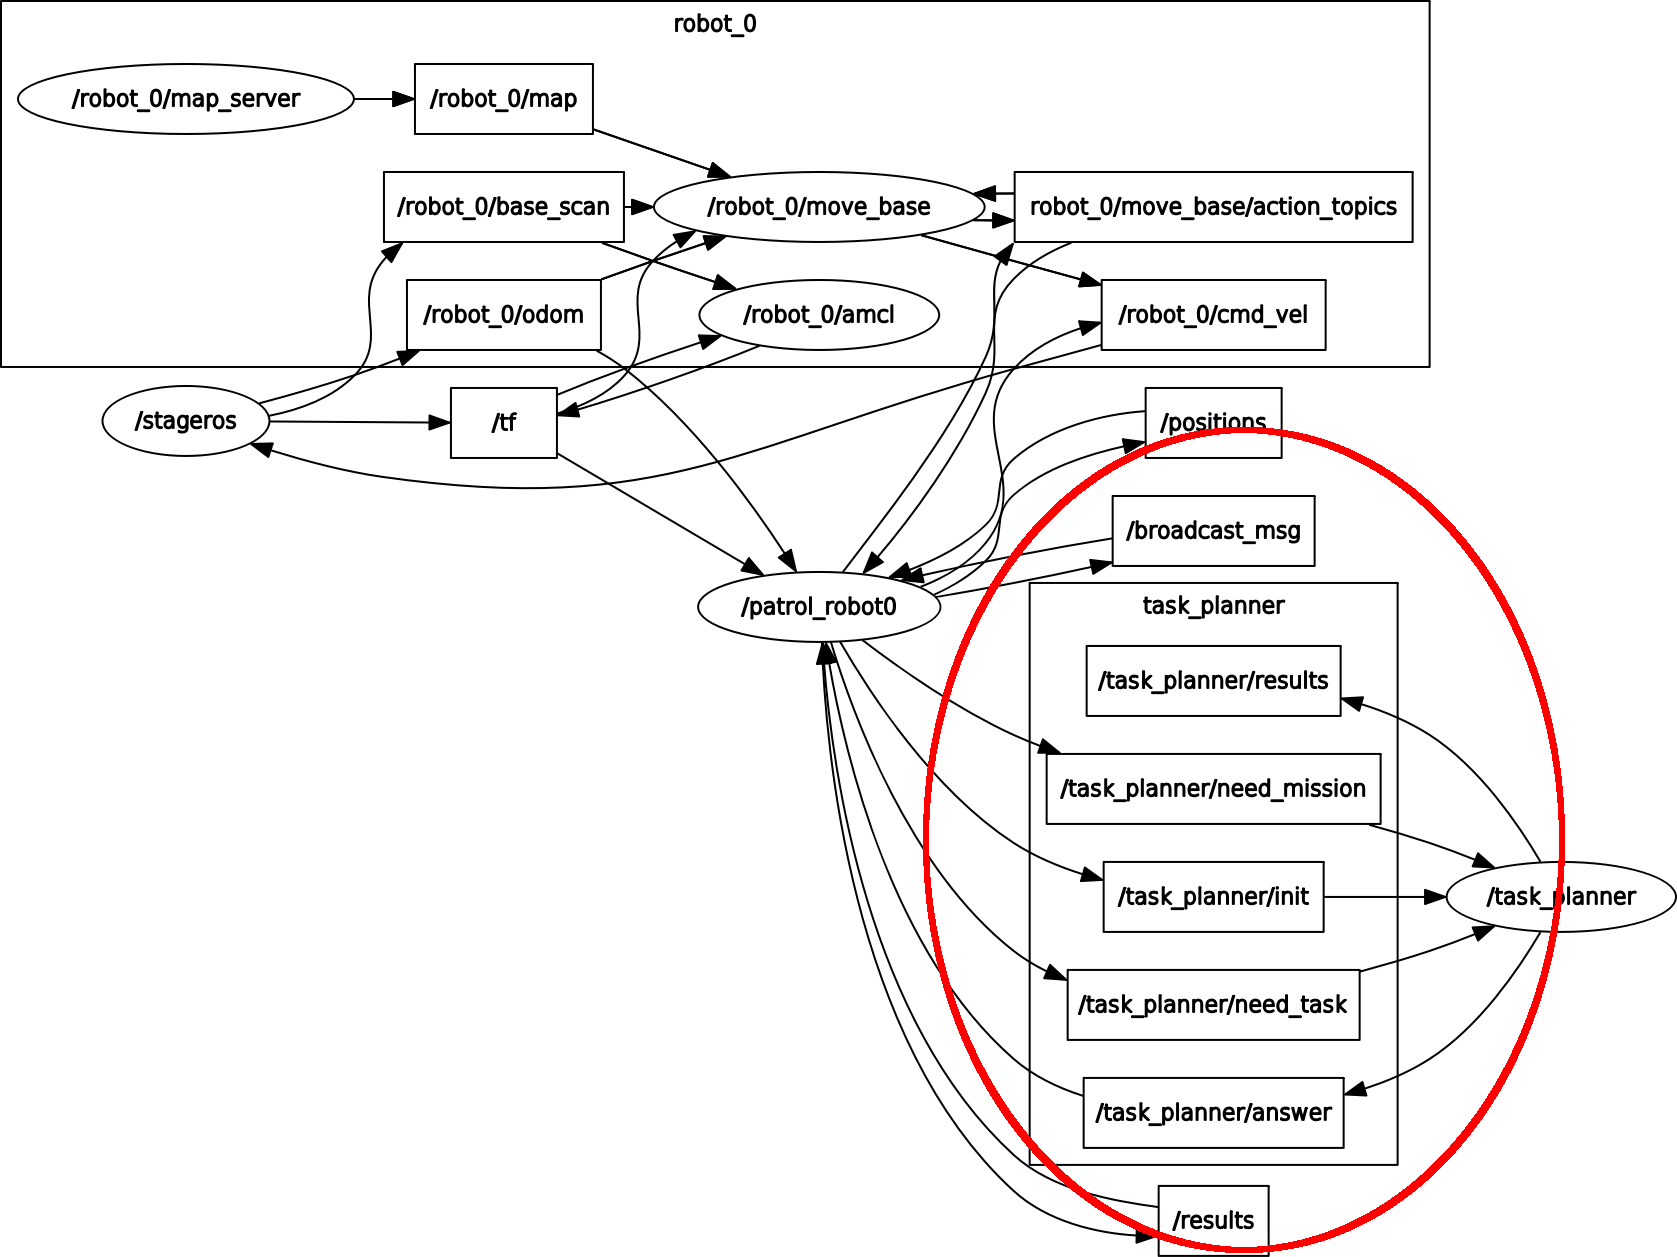
\includegraphics[scale=0.25]{img/rosgraph}
        \end{figure}
    \end{frame}


    \begin{frame}[fragile]{Video}
    \centering
    \includemedia[height=0.7\linewidth,width=1\linewidth,activate=pageopen,
    passcontext,
    transparent,
    addresource=video/video.mp4,
    flashvars={source=video/video.mp4}
    ]{}{VPlayer.swf}
    \end{frame}

    \begin{frame}[fragile]{Empirical Results}
        The {\bf configuration} is based on the size of the task set $\mathcal{T}$, the robot's {\bf capacity} and number of the {\bf team} robots.

        We performed 260 experiments with 18 different settings.
        \begin{table}[hbt]
         \resizebox{\linewidth}{2.5cm}{
        \begin{tabular}{|c|c|c|c|c|c|} \hline
            {\bf Configuration} & {\bf Algorithm} & {\bf $ \overline{Time}$} & {\bf $\overline{Interference}$} & {\bf $\overline{Distance}$} & {\bf $\bar{\sigma}(Distance)$}         \\ \hline
            6/-/4               &  \srst          & {\color{blue}{124.52}}$[\pm 3.12]$        & 42      & {\color{blue}{2194.75 }}&  114.2 \\ \hline
            6/3/4               & \gsp            & {\color{red}{117.44}}$[\pm 1.85]$        & 35.75    & {\color{red}{1769 }}& 43.83  \\ 
                                & {\bf \sps} & {\bf 115.28}$[\pm 4.10]$        & {\bf 33.5}   & {\bf 1702.5 }& {\bf 23.67}  \\ \hline
            6/5/4               & \gsp            &  {\color{red}{93.4}} $[\pm 1.01]$         & 29       & {\color{red}{1688.5 }}&  34.5   \\
                                & {\bf \sps}      & {\bf 91.8}$[\pm 2.14]$        & {\bf 30.75 }  & {\bf 1546.5}& {\bf 35.8}  \\ \hline
            9/-/4               &  \srst          & {\color{blue}{178.55}}$[\pm 4.23]$    & 52           & {\color{blue}{2755.75}}& 135.8 \\ \hline
            9/3/4               & \gsp           & {\color{red}{152.55}}$[\pm 2.87]$     & 46.75        & {\color{red}{2200 }}& 113.4 \\ 
                               & {\bf \sps}            & {\bf 134.23}$[\pm 3.25]$     &  {\bf 40.63}     & {\bf 2182.5}& {\bf 27} \\ \hline
            9/5/4              & \gsp           &  {\color{red}{134.23}}$[\pm 3.26]$        & 40.6      & {\color{red}{2098.3}}  &   93.45    \\
                               & {\bf \sps}           &  {\bf 93.05}$[\pm 5.15]$         & {\bf 32.25}   & {\bf 1530.25 }&   {\bf 0} \\ \hline    
            21/-/4              &  \srst          & {\color{blue}{402.12}}$[\pm 5.06]$     & 132.25      & {\color{blue}{6232.35 }}&  295.1 \\ \hline
            21/3/4              & \gsp           & {\color{red}{343.23}}$[\pm 6.10]$ & 98.23            & {\color{red}{5231.25 }}& 342.2   \\ 
            21/5/4              & \gsp           & {\color{red}{294.40}}$[\pm 7.60]$ & 77.63            & {\color{red}{4683.25 }}& 367.5  \\ \hline
        \end{tabular}}
    \end{table}
       
    \end{frame}



    \begin{frame}[fragile]{Conclusions and Future Work}
        In conclusion: 
        \begin{itemize}
            \item The results respects the expectations.
            \item The quality of solutions found by GSP is comparable with the 
            quality of solutions found by SPS.
            \item GSP problem can approximate the results 
            of a SPS problem in {\bf less} time.
        \end{itemize}
        We focus on a {\bf centralized coordinator}.Future works we want to 
        perform a {\bf distributed coordiantion}.

    Allocation strategy should be more {\bf flessible}, {\bf adaptive} to traffic then {\bf fault-tolenace}. 
    \end{frame}

    \begin{frame}
        \begin{center}
        {\bf Thank you for your attention!}
        \end{center}
    \end{frame}

  
      \begin{frame}[fragile]{ROS package Logistic\_sim}
        \begin{figure}[hbt]
            \centering
            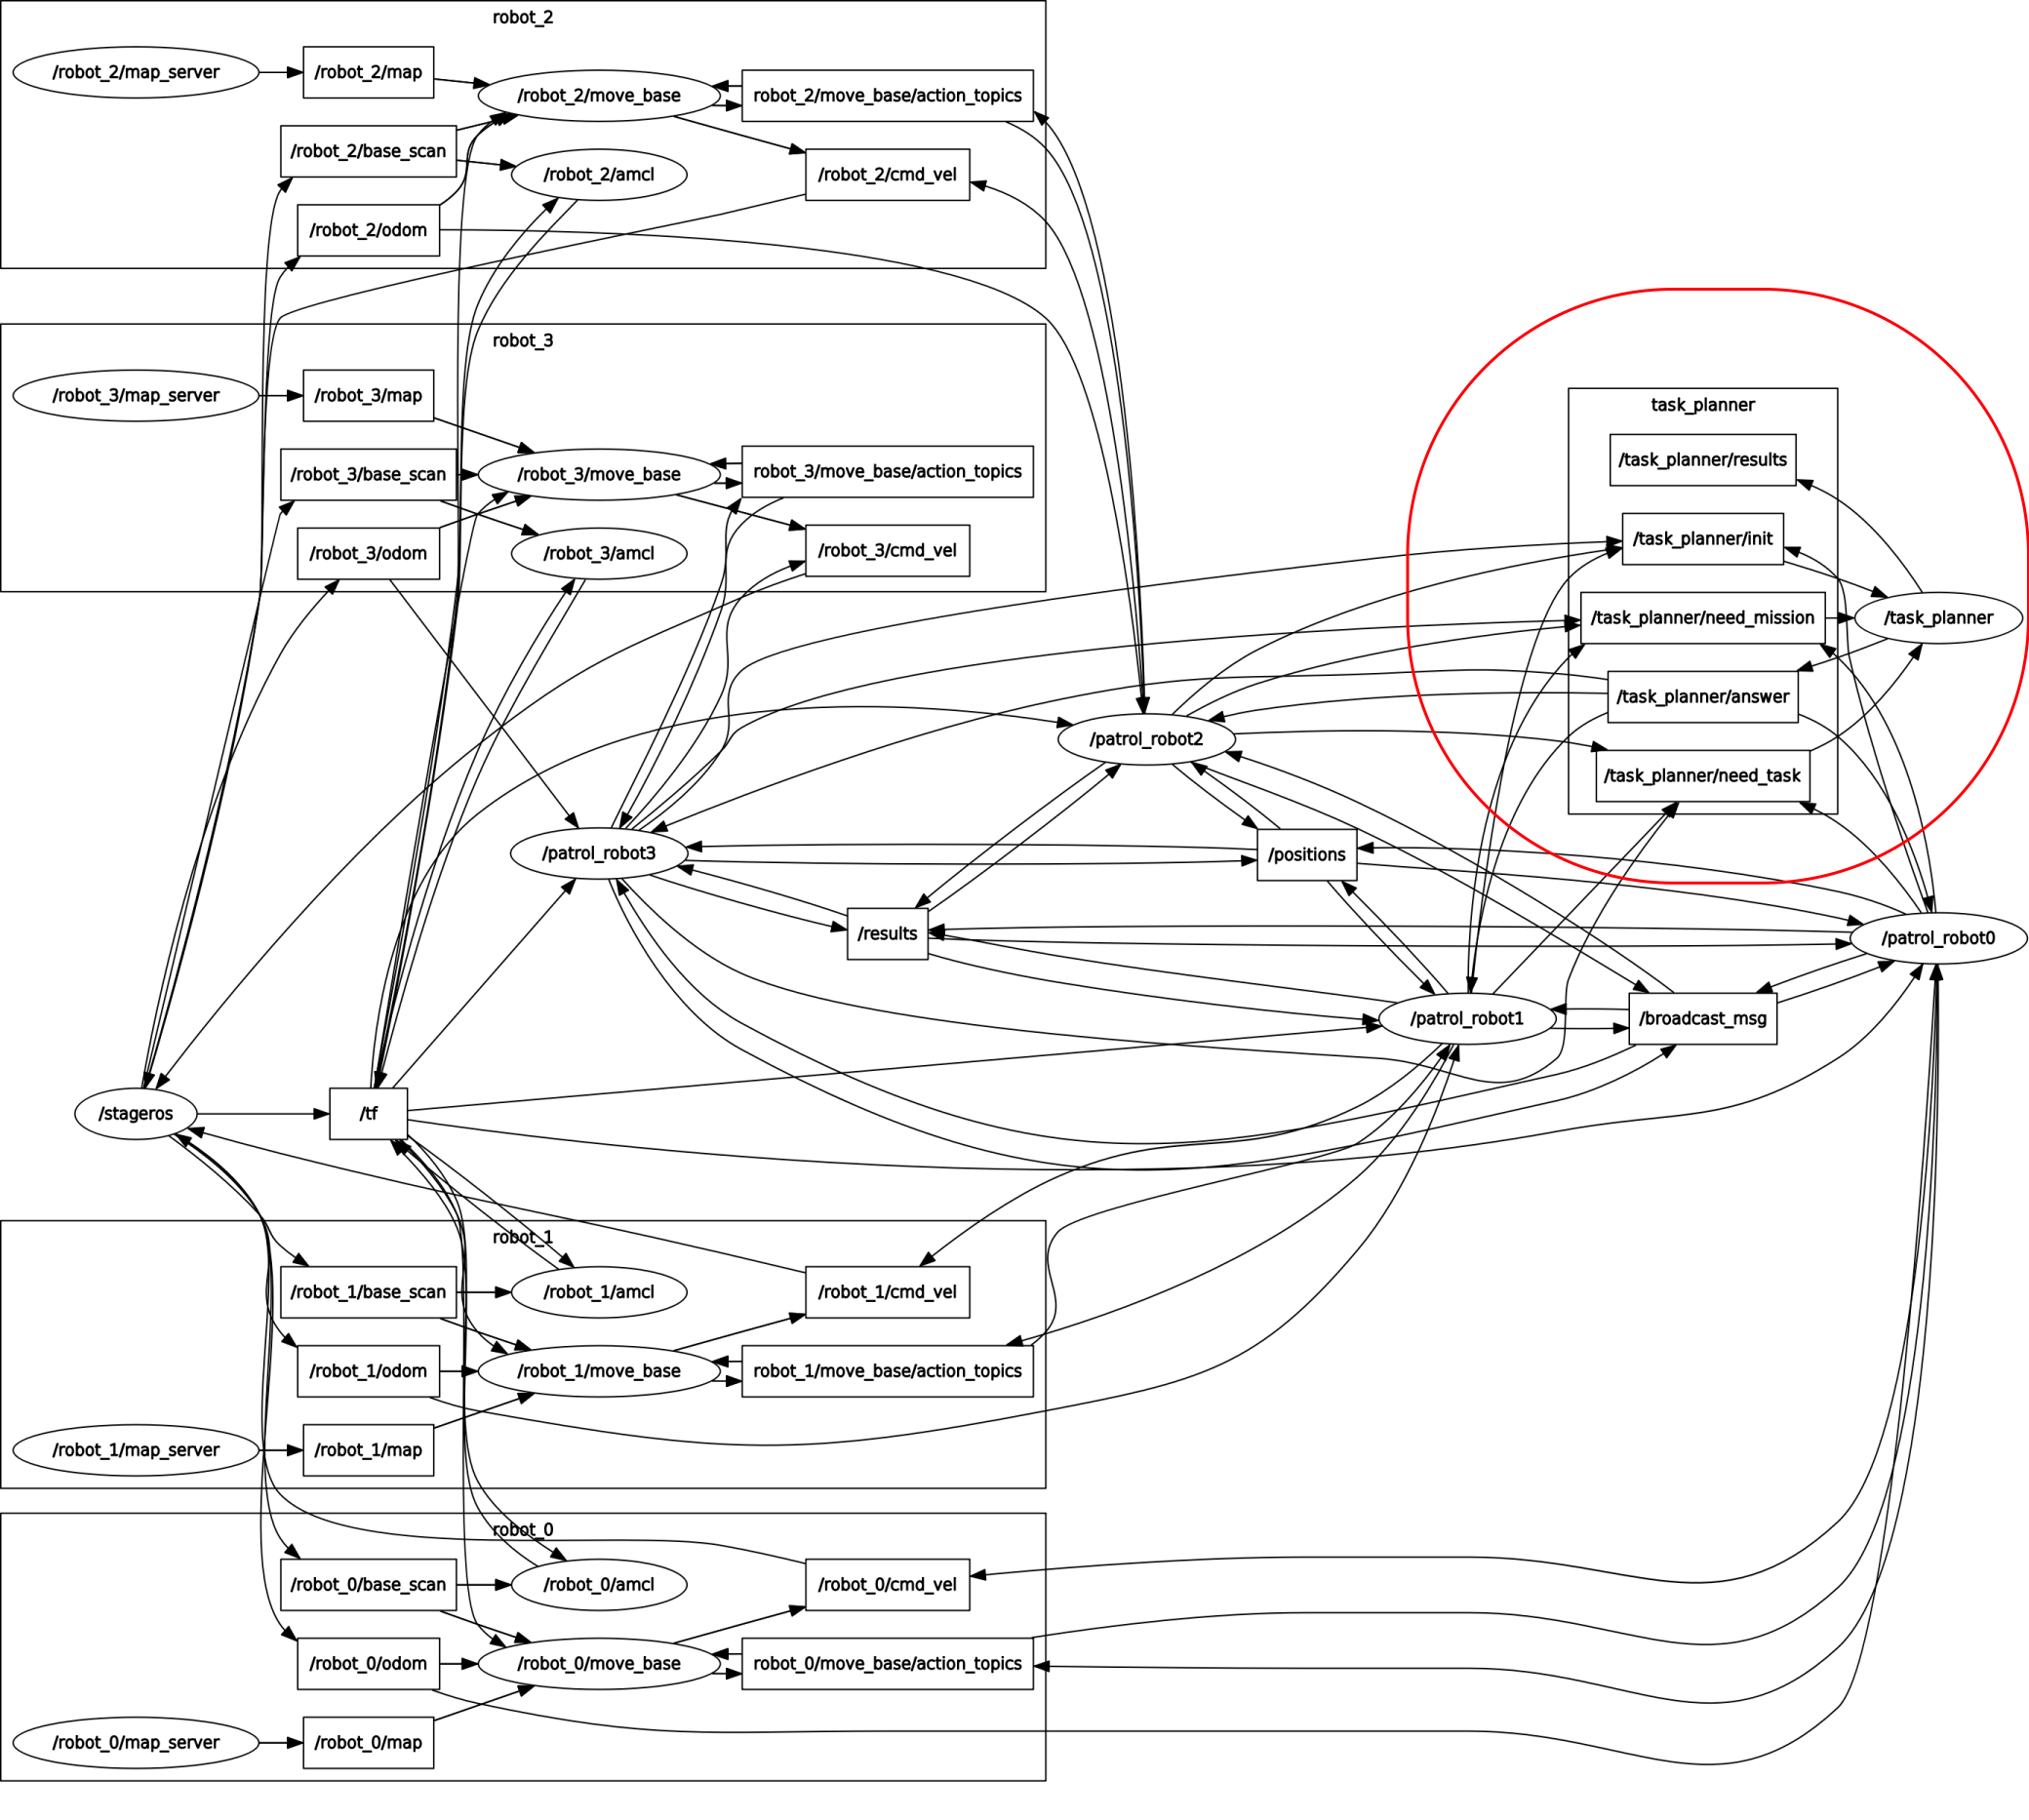
\includegraphics[scale=0.12]{img/rosgraph1}
        \end{figure}
    \end{frame}

    \begin{frame}{Stage 2D}
        \begin{figure}[hbt]
            \centering
            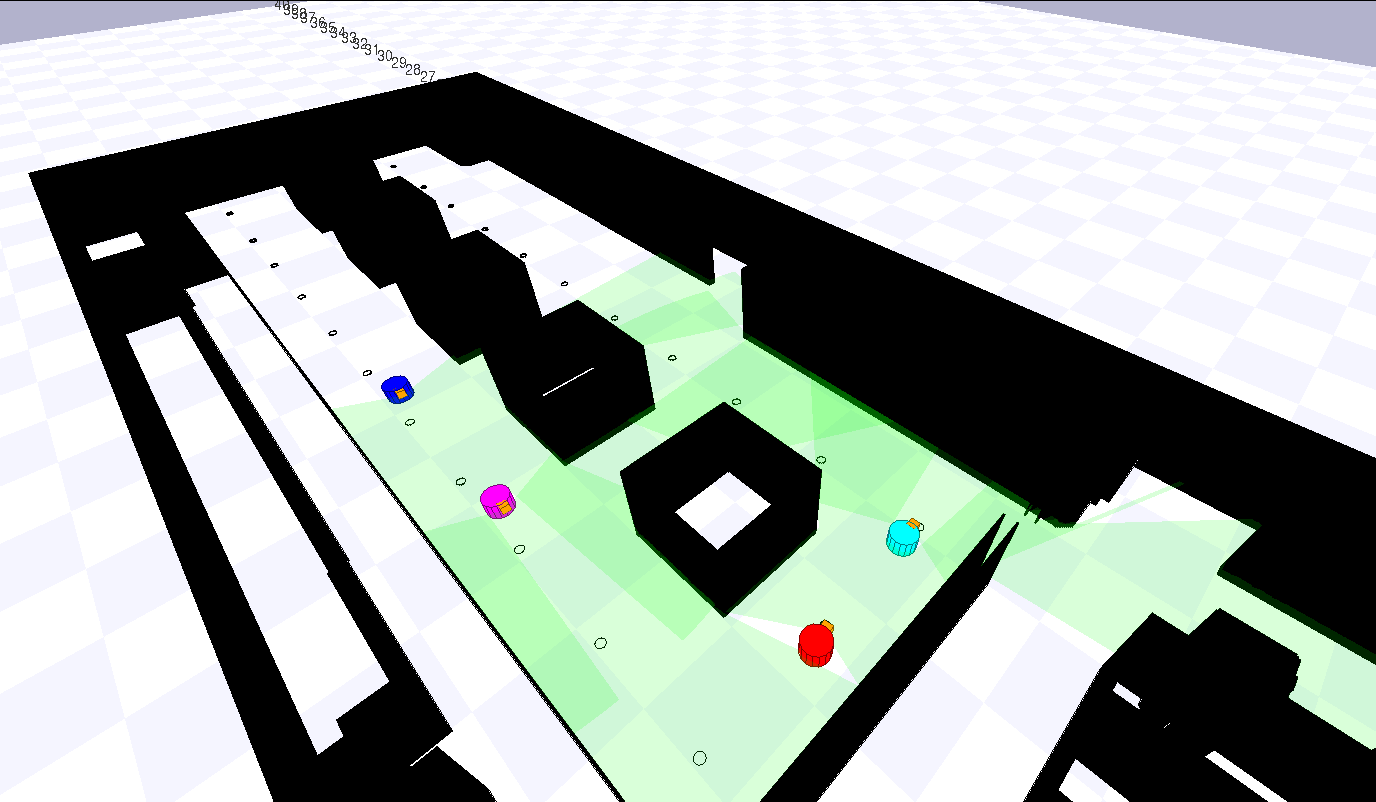
\includegraphics[width=\textwidth]{img/prospective}
        \end{figure}
    \end{frame}

    \begin{frame}[fragile]{All Results}
        \resizebox{\linewidth}{4.3cm}{
        \begin{tabular}{|c|c|c|c|c|c|} \hline
            {\bf Configuration} & {\bf Algorithm} & {\bf $ \overline{Time}$} & {\bf $\overline{Interference}$} & {\bf $\overline{Distance}$} & {\bf $\bar{\sigma}(Distance)$}         \\ \hline
            6/-/2               & {\bf \srst}           & {\color{blue}{218.32}}$[\pm 6.19]$        & 63.45   & {\color{blue}{3747.90}} &  87.8\\ \hline 
            6/3/2               & \gsp            & {\color{red}{194.52}}$[\pm 6.42]$        & 49.65    & {\color{red}{3401.15}} & 251.37  \\ 
                                & \textsl{\sps}            & {\color{green}{177.00}}$[\pm 1.99]$        & 49.34  & {\color{green}{3132.5 }}& {\bf 0}  \\ \hline
            6/5/2               & \gsp            & {\color{red}{142.08}}$[\pm 1.39]$       &   42.2    & {\color{red}{2714.25  }}    &  206.43  \\
                                & \textsl{\sps}            & {\color{green}{138.98}}$[\pm 2.41]$       &  39.38  & {\color{green}{ 2601.25 }} &  156.47   \\ \hline
            6/-/4               & {\bf \srst}           & {\color{blue}{124.52}}$[\pm 3.12]$        & 42      & {\color{blue}{2194.75 }}&  114.2 \\ \hline
            6/3/4               & \gsp            & {\color{red}{117.44}}$[\pm 1.85]$        & 35.75    & {\color{red}{1769 }}& 43.83  \\ 
                                & \textsl{\sps}            & {\color{green}{115.28}}$[\pm 4.10]$        & 33.5   & {\color{green}{1702.5 }}& 23.67  \\ \hline
            6/5/4               & \gsp            & {\color{red}{ 93.4}}$[\pm 1.01]$         & 29       & {\color{red}{1688.5 }}&  34.5   \\
                                & \textsl{\sps}            & {\color{green}{ 91.8}}$[\pm 2.14]$        & 30.75   & {\color{green}{1546.5 }}& 35.8  \\ \hline
            9/-/2               & {\bf \srst}           & {\color{blue}{292.24}}$[\pm 3.06]$      &  85.5     & {\color{blue}{5201.5 }}& 34.76\\ \hline
            9/3/2              & \gsp            & {\color{red}{265.72}}$[\pm 2.64]$      & 71.5        & {\color{red}{4491.5  }}& {\bf 0}  \\ 
                               & \textsl{\sps}            & {\color{green}{240.74}}$[\pm 10.42]$        & 75.5   & {\color{green}{4232.5 }}& 310.43 \\ \hline
             9/5/2             & \gsp            & {\color{red}{232.84}}$[\pm 4.71]$      &  68.85      & {\color{red}{ 4041.25 }} &  236 \\
                               & \textsl{\sps}            & {\color{green}{168.34}}$[\pm 2.03]$       &   50.5   & {\color{green}{3132.5 }}& {\bf 0 } \\ \hline 
            9/-/4               & {\bf \srst}          & {\color{blue}{178.55}}$[\pm 4.23]$    & 52           & {\color{blue}{2755.75}}& 135.8 \\ \hline
            9/3/4               & \gsp           & {\color{red}{152.55}}$[\pm 2.87]$     & 46.75        & {\color{red}{2200 }}& 113.4 \\ 
                               & \textsl{\sps}            & {\color{green}{134.23}}$[\pm 3.25]$     &  40.63     & {\color{green}{2182.5 }}& 27 \\ \hline
            9/5/4              & \gsp           &  {\color{red}{134.23}}$[\pm 3.26]$        & 40.6      & {\color{red}{2098.3   }}  &   93.45    \\
                               & \textsl{\sps}           &  {\color{green}{93.05}}$[\pm 5.15]$         & 32.25   & {\color{green}{1530.25 }}&   {\bf 0} \\ \hline    
            21/-/2             & {\bf \srst}           & {\color{blue}{629.10}}$[\pm 8.84]$        & 154.6    & {\color{blue}{11773.5 }}&  229.75 \\ \hline
            21/3/2              & \gsp           & {\color{red}{561.93}}$[\pm 8.00]$     &  134.3       & {\color{red}{10133.16 }}&  201.2   \\ 
      21/5/2              & \gsp           & {\color{red}{497.45}}$[\pm 6.15]$      & 126         & {\color{red}{9079}} & 210.4  \\ \hline
            21/-/4              & {\bf \srst}          & {\color{blue}{402.12}}$[\pm 5.06]$     & 132.25      & {\color{blue}{6232.35 }}&  295.1 \\ \hline
            21/3/4              & \gsp           & {\color{red}{343.23}}$[\pm 6.10]$ & 98.23            & {\color{red}{5231.25 }}& 342.2   \\ 
            21/5/4              & \gsp           & {\color{red}{294.40}}$[\pm 7.60]$ & 77.63            & {\color{red}{4683.25 }}& 367.5  \\ \hline
        \end{tabular}}
    \end{frame}










